%\documentclass[aps,onecolumn,preprint,superscriptaddress,nofootinbib,floats]{revtex4}
%\usepackage{graphicx}

\documentclass[12pt]{article}

\usepackage{amsmath}
\usepackage[linesnumbered,ruled,noline,noend]{algorithm2e}

%\usepackage[linesnumbered,noline,noend]{algorithm2e}
%\usepackage{amsmath}

\SetNlSty{}{}{}

\let\oldnl\nl% Store \nl in \oldnl
\newcommand\nonl{%
  \renewcommand{\nl}{\let\nl\oldnl}}% Remove line number for one line



\def\beq{\begin{equation}}
\def\eeq{\end{equation}}


\usepackage{amsmath,amssymb,graphicx,multirow,xspace,slashed}
\usepackage[colorlinks=true,urlcolor=blue,anchorcolor=blue,citecolor=blue,filecolor=blue,linkcolor=blue,menucolor=blue,pagecolor=blue]{hyperref}


\usepackage{floatrow}
% Table float box with bottom caption, box width adjusted to content
\newfloatcommand{capbtabbox}{table}[][\FBwidth]


\usepackage[font=footnotesize,labelfont=bf]{caption}

\newcommand*\myat{{\fontfamily{ptm}\selectfont @}}

%\usepackage[notref]{showkeys}
\usepackage{lineno}

\allowdisplaybreaks
\bibliographystyle{JHEP}

\addtolength{\oddsidemargin}{-.4in}
\addtolength{\evensidemargin}{-.4in}
\addtolength{\textwidth}{0.8in}
\addtolength{\topmargin}{-.6in}
\addtolength{\textheight}{1in}
%\addtolength{\footskip}{0.3in}
\renewcommand{\baselinestretch}{1.2}

\long\def\symbolfootnote[#1]#2{\begingroup%
\def\thefootnote{\fnsymbol{footnote}}\footnote[#1]{#2}\endgroup}

\renewcommand{\textfraction}{0}
\renewcommand{\topfraction}{0.95}


\newcommand{\newc}{\newcommand}
\newc{\gsim}{\lower.7ex\hbox{$\;\stackrel{\textstyle>}{\sim}\;$}}
\newc{\lsim}{\lower.7ex\hbox{$\;\stackrel{\textstyle<}{\sim}\;$}}
\newc{\gev}{\,{\rm GeV}}
\newc{\mev}{\,{\rm MeV}}
\newc{\ev}{\,{\rm eV}}
\newc{\kev}{\,{\rm keV}}
\newc{\tev}{\,{\rm TeV}}

\newcommand{\ifb}{\,\mathrm{fb}^{-1}}
\newcommand{\ipb}{\,\mathrm{pb}^{-1}}
\renewcommand*\descriptionlabel[1]{\hspace\labelsep\normalfont #1}

\def\ln{\mathop{\rm ln}}
\def\tr{\mathop{\rm tr}}
\def\Tr{\mathop{\rm Tr}}
\def\Im{\mathop{\rm Im}}
\def\Re{\mathop{\rm Re}}
\def\bR{\mathop{\bf R}}
\def\bC{\mathop{\bf C}}
\def\lie{\mathop{\hbox{\it\$}}} %pound sterling
\newc{\mz}{M_Z}
\newc{\mpl}{M_*}
\newc{\mw}{m_{\rm weak}}
\newc{\nr}[1]{N^c_R{}_{#1}}

%\renewcommand{\phi}{\varphi}

%indices and other greek stuff
\renewcommand{\a}{\alpha}
\newcommand{\da}{{\dot \alpha}}
\renewcommand{\b}{\beta}
\newcommand{\db}{{\dot\beta}}
\newcommand{\g}{\gamma}
\newcommand{\dg}{{\dot\gamma}}
\renewcommand{\d}{\delta}
\newcommand{\dd}{{\dot\delta}}
\newcommand{\m}{\mu}
\newcommand{\n}{\nu}
\newcommand{\e}{\epsilon}
\newcommand{\s}{\sigma} 
\renewcommand{\r}{\rho}
\newcommand{\bs}{{\bar\sigma}}
\renewcommand{\l}{\lambda}
\renewcommand{\L}{\Lambda}
\renewcommand{\k}{\kappa}
\renewcommand{\th}{\theta}
\newcommand{\thb}{{\bar\theta}}
\newcommand{\D}{\Delta}
\newcommand{\B}{\bar B_\mu}
\newcommand{\cA}{c_{A_{u,d}}}
\newcommand{\cH}{c_{m_{u,d}}}
\renewcommand{\dag}{\dagger}
\newcommand{\bra}{\langle}
\newcommand{\ket}{\rangle}
\newcommand{\Q}{\bar Q}
\renewcommand{\O}{O}

\newcommand{\CM}{{\mathcal M}}

%%%%%%%%%%%%%%%%%%%%%%%% special abrev's %%%%%%%%%%%%%%%%%%%%%%%%%%%%%

\newcommand{\mhu}{{\hat m_{H_u}}}
\newcommand{\mhd}{{\hat m_{H_d}}}
\newcommand{\mhud}{{\hat m_{H_{u,d}}}}


%%%%%%%%%%%%%%%%%%%%%%% latex eqn abrev's %%%%%%%%%%%%%%%%%%%%%%%%%%%%

\def\beq{\begin{equation}}
\def\eeq{\end{equation}}
\newcommand{\bea}{\begin{eqnarray}\begin{aligned}}
\newcommand{\eea}{\end{aligned}\end{eqnarray}}
\def\bitem{\begin{itemize}}
\def\eitem{\end{itemize}}
%
%
%%%%%%%%%%%%%%%%%%%%%%% common abrev's %%%%%%%%%%%%%%%%%
%
%

\newc{\ie}{{\it i.e.}}          \newc{\etal}{{\it et al.}}
\newc{\eg}{{\it e.g.}}          \newc{\etc}{{\it etc.}}
\newc{\cf}{{\it c.f.}}
\newcommand{\kahler}{K\"{a}hler }

\newcommand{\lang}{\mathcal{L}}
\newcommand{\C}{\mathbb{C}}
\newcommand{\CO}{O}
\newcommand{\half}{\frac{1}{2}}


%\renewcommand{\epvar}{\varepsilon}
%\renewcommand{\phi}{\varphi}
\renewcommand{\topfraction}{0.85}
\renewcommand{\textfraction}{0.1}
\renewcommand{\floatpagefraction}{0.75}

%number equations by section
 %\numberwithin{equation}{section}

%toc depth
\setcounter{tocdepth}{2}

%Begin special definitions for Instructions file
\newcommand{\ttbs}{\char'134}%\backslash for \tt
\newcommand\fverb{\setbox\fverbbox=\hbox\bgroup\verb}
\newcommand\fverbdo{\egroup\medskip\noindent%
            \fbox{\unhbox\fverbbox}\ }
\newcommand\fverbit{\egroup\item[\fbox{\unhbox\fverbbox}]}
\newbox\fverbbox
\newcommand{\jhepname}{JHEP}
%end


\renewcommand{\arraystretch}{1.3}

%\usepackage[usenames,dvipsnames]{xcolor}


\usepackage{tikz}

\newcommand{\shrug}[1][]{%
\begin{tikzpicture}[baseline,x=0.8\ht\strutbox,y=0.8\ht\strutbox,line width=0.125ex,#1]
\def\arm{(-2.5,0.95) to (-2,0.95) (-1.9,1) to (-1.5,0) (-1.35,0) to (-0.8,0)};
\draw \arm;
\draw[xscale=-1] \arm;
\def\headpart{(0.6,0) arc[start angle=-40, end angle=40,x radius=0.6,y radius=0.8]};
\draw \headpart;
\draw[xscale=-1] \headpart;
\def\eye{(-0.075,0.15) .. controls (0.02,0) .. (0.075,-0.15)};
\draw[shift={(-0.3,0.8)}] \eye;
\draw[shift={(0,0.85)}] \eye;
% draw mouth
\draw (-0.1,0.2) to [out=15,in=-100] (0.4,0.95); 
\end{tikzpicture}}



\newcommand{\MYhref}[3][blue]{\href{#2}{\color{#1}{#3}}}%

\begin{document}
%
%\title{Toy Generative Model for Jets}
%\author{Kyle Cranmer, Sebastian Macaluso and Duccio Pappadopulo}
%\maketitle


\begin{center}

\vskip 1cm
{\Large \bf Toy Generative Model for Jets}

\vskip 1.0cm
{\large $\text{Kyle Cranmer}^1$, $\text{Sebastian Macaluso}^1$ and $\text{Duccio Pappadopulo}^2$}
\vskip 0.6cm
{\small \it 1 Center for Cosmology and Particle Physics $\&$ Center for Data Science, New York University, USA} \\
{\small \it 2 Bloomberg LP, New York, NY 10022, USA.}
\vskip 2.0cm

\end{center}




\section{Introduction}

In this notes, we provide a standalone description of a generative model to aid in machine learning (ML) research for jet physics. The motivation is to build a model that has a tractable likelihood, and is as simple and easy to describe as possible but at the same time captures the essential ingredients of parton shower generators in full physics simulations.  The aim is for the model to have a python implementation with few software dependencies.

Parton shower generators are software tools that encode a physics model for the simulation of jets that are produced at colliders, e.g. the Large Hadron Collider at CERN.
Jets are a collimated spray of energetic charged and neutral particles. Parton showers generate the particle content of a jet, going through a cascade process, starting from an initial unstable particle. In this description, there is a recursive algorithm that produces binary splittings of an unstable parent particle into two children particles, and a stopping rule. Thus, starting from the initial unstable particle, successive splittings are implemented until all the particles are stable (i.e. the stopping rule is satisfied for each of the final particles). We refer to this final particles as the jet constituents.

As a result of this {\it showering process}, there could be many latent paths that may lead to a specific jet (i.e. the set of constituents). Thus, it is natural and straightforward to represent a jet and the particular showering path that gave rise to it as a binary tree, where the inner nodes represent each of the unstable particles and the leaves represent the jet constituents.  


% =====================================================
\vspace{0.6cm}
\section{Model description}

Our model implements a recursive algorithm to generate a binary tree, whose leaves are the jet constituents. Jet constituents in full physics simulations are described in terms of a 4 dimensional vector that specifies their energy $E$ and spatial momentum $\vec{p}$, which determines the direction of motion. 
We want our model to represent the following features:
%There is a set of physics features that we want our model to represent, and they are described as follows:
\begin{itemize}
\item Momentum conservation: the total momentum of the jet (the momentum of the root of the tree) is obtained from adding the momentum of all of its constituents.

\item Running of the splitting scale $\Delta$: each splitting is characterized by a scale that decreases when evolving down the tree from root to leaves.




% and $p_{\text{T}}$ is the momentum transverse to some fixed direction. 
%Also, $\alpha=\{-1,0,1\}$ defines the $\{\text{anti-kt, CA and kt}\}$ clustering algorithms respectively. 

\end{itemize}

We also want our model to lead to a natural analogue of the generalized $k_t$ clustering algorithms for the generated jets. These algorithms are characterized by

\begin{itemize}
\item Permutation invariance: the jet momentum should be invariant with respect to the order in which we cluster its constituents.

\item Distance measure: the angular separation between two jet constituents is typically used as a distance measure among them. In particular, traditional jet clustering algorithms are based on a measure given by 
$d_{ij} \propto  \Delta R_{ij}^2$
where $\Delta R_{ij}$ is the angular separation between two particles.

\end{itemize} 

As a result, we build our model as follows. Each node of the jet tree represents a particle and encodes its momentum vector. During the generative process, starting from the root of the tree, each parent node is split, generating a left (L) and a right (R) child. The L (R) child's momentum is obtained from subtracting (adding) a vector of magnitude $\Delta$ to half of the parent's momentum vector. This prescription ensures {\it momentum conservation} and {\it permutation invariance}.

We consider a 2D model to be able to define an angular {\it distance measure}. Also, the angular separation between a parent and its L/R child's momentum is expected to decrease as the physics shower moves forward from the root to the leaves of the tree. The magnitude of the momentum of each node is also expected to drop in the same way, i.e. ``the radiation gets softer when evolving down the tree".
Both requirements are satisfied by the {\it running of the splitting scale $\Delta$}, which we achieve by rescaling the value of $\Delta$ by a factor $r$. ($r$ is drawn from a decaying exponential distribution each time a new splitting is produced.)  
This way, we also assign a $\Delta$ value to each node of the tree. 


We build our 2D model in the $(y,z)$ plane, where $\hat{z}$ is the direction of the beam axis and $\hat{y}$ the transverse direction.\footnote{At the Large Hadron Collider, jets are produced from the collision of two beams of protons moving in opposite directions.} 
We define the transverse momentum as $p_{\text{T}} =|p_y|$. We show in Fig.~\ref{fig:1DTree} a tree visualization plot of a sample jet generated with our model.

\begin{figure*}
{
  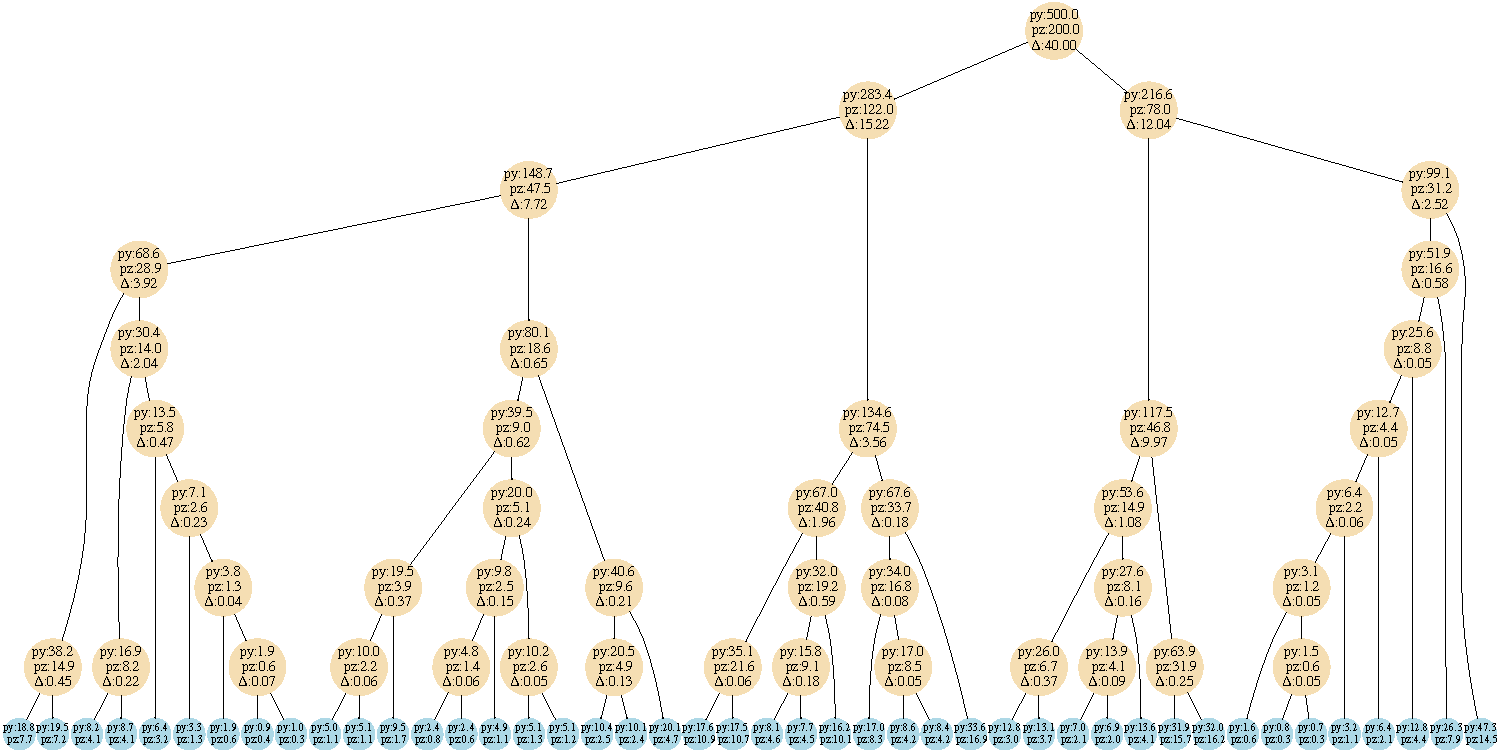
\includegraphics[width=\linewidth]{plots/figTruth_jet9.pdf}
%  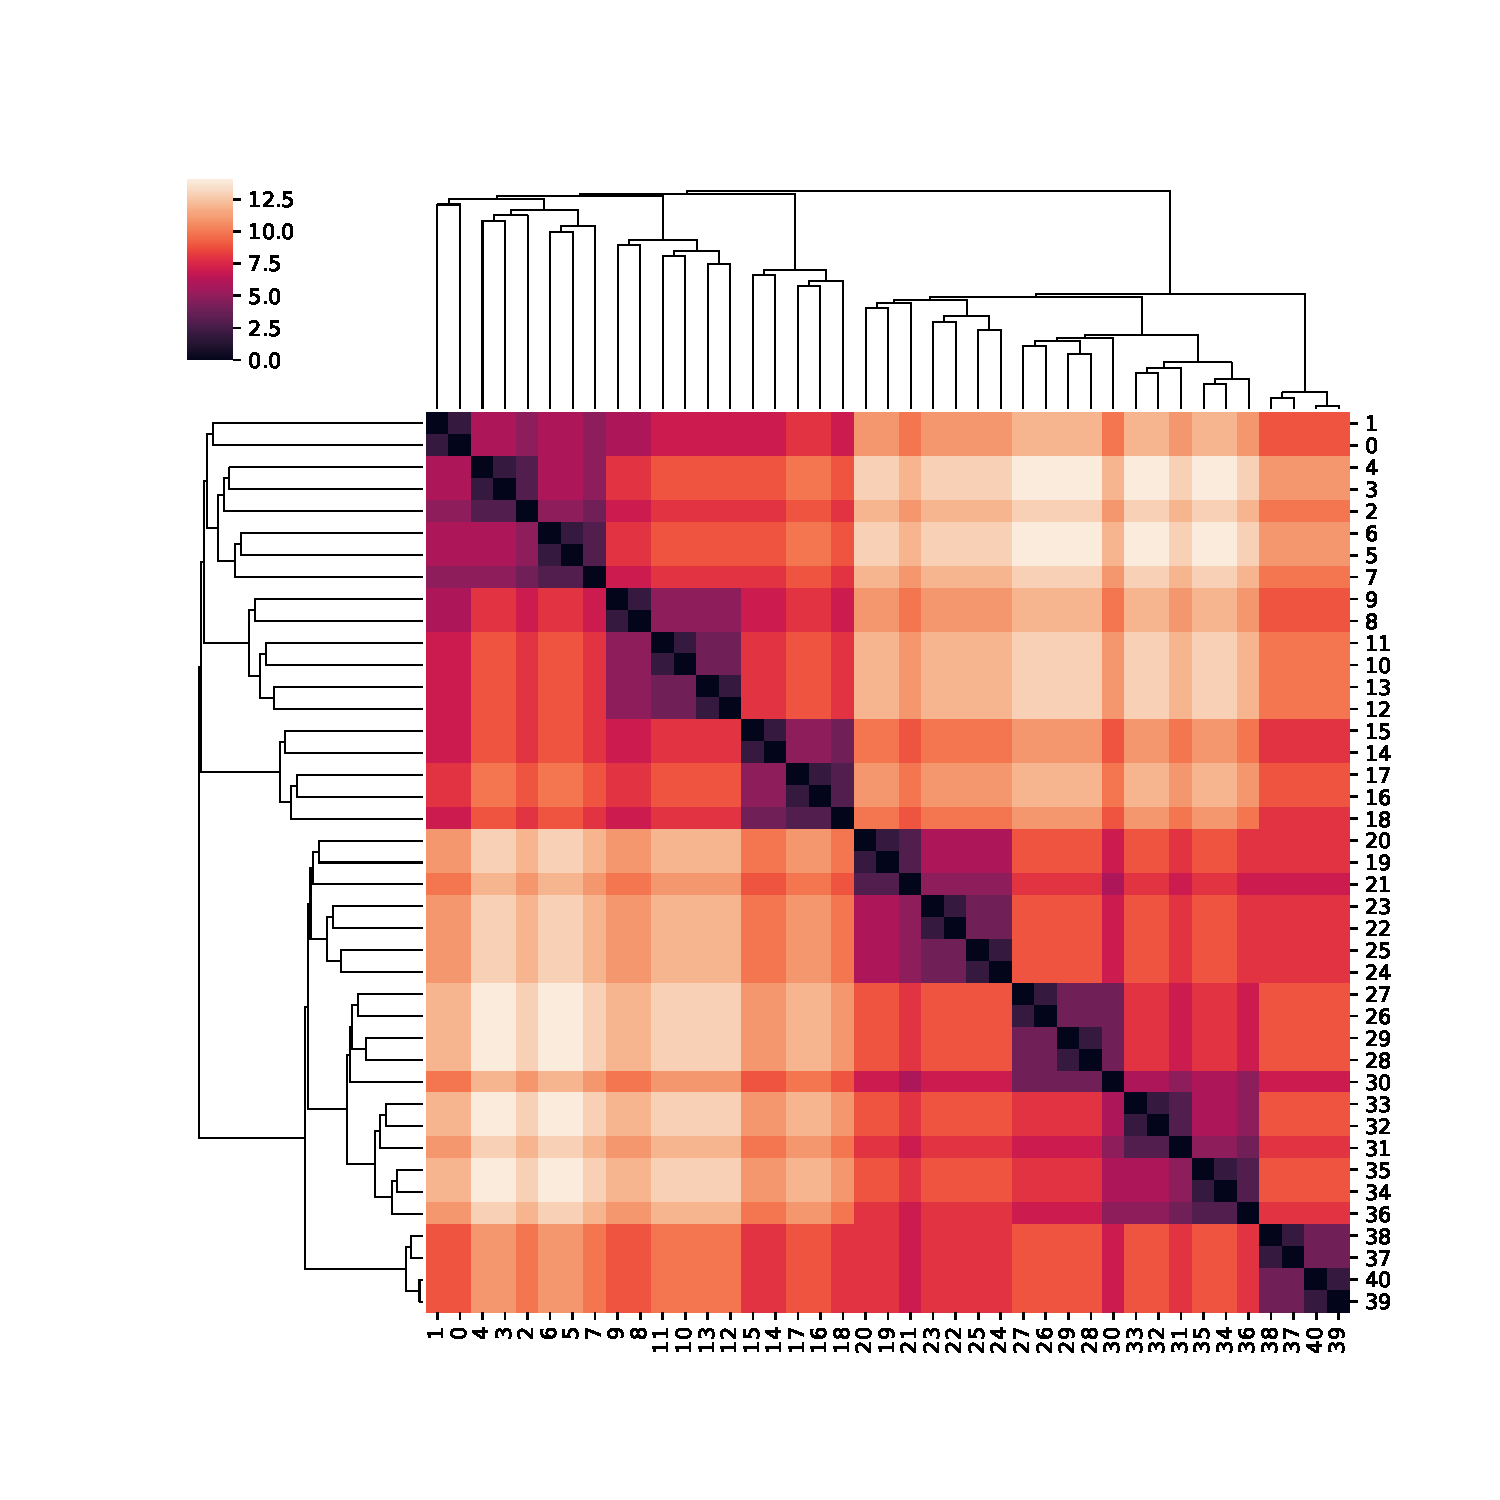
\includegraphics[width=0.5\linewidth]{plots/figTruthTruth_fullpath_jet2}
}
\caption{\small{Tree visualization of a sample jet generated with our model that represents a W boson jet, as described in section \ref{Heavy resonance vs QCD like jet}. We show the values of $\vec{p} =(p_y,p_z)$ for each node and the scale $\Delta$ for the splitting of the inner nodes. The horizontal ordering of the leaves corresponds to the order in which the leaves are accessed when traversing the tree (and is not related to the particle momentum $\vec{p}$).
}}
\label{fig:1DTree}
\end{figure*}

%%-------------
\subsection{Generative process}

In this section, we describe the implementation of the generative process, which depends on the following input parameters:
\begin{itemize}

\item $\vec{p}_0$: momentum of the jet. This will be the input value for the root node of the tree.
\item $\lambda$: decaying rate for the exponential distribution.
\item $\Delta_0$: Initial scale of the splitting. 
\item $\Delta_\text{cut}$: cut-off scale to stop the showering process. 

\end{itemize}

Next, we describe the splitting of a node.
%\subsubsection{Splitting of a node}
Given a parent node with momentum $\vec{p}_\text{p}$, and a scalar value $\Delta_{\text{p}}$ that sets the scale of the splitting, we define the splitting function as follows:
\begin{enumerate}

\item We draw a value $\phi_\text{p}$ for the angle in the (y,z) plane, from a uniform distribution in the range $\{0,2\pi\}$ and define
\bea\label{eq:Deltavec}
\vec{\Delta}_\text{p}= \Delta_\text{p}\,\,(\sin\phi_\text{p},\cos\phi_\text{p})
\eea 

\item We obtain the L,R children nodes momentum,
\bea\label{eq:pLR}
\vec{p}_\text{L}= \frac{1}{2} \vec{p}_\text{p} - \vec{\Delta}_\text{p}  \\
\vec{p}_\text{R}= \frac{1}{2} \vec{p}_\text{p} +\vec{\Delta}_\text{p}
\eea

\item We separately draw $r_\text{L}$ and $r_\text{R}$ from an exponential distribution 
\bea \label{eq:exponential}
f(r | \lambda)=\lambda e^{-\lambda r} 
\eea

and generate
\bea
\Delta_\text{L} &= \Delta_\text{p} \,\, r_\text{L}\\
\Delta_\text{R} &= \Delta_\text{p} \,\, r_\text{R}
\eea

\end{enumerate}



We start the showering process with the root node as the parent node and build the jet binary tree recursively as follows:
\begin{itemize}

\item We split the parent node, and get $\vec{p}_\text{L}$, $\vec{p}_\text{R}$, $\Delta_\text{L}$, $\Delta_\text{R}$.

\item If $\Delta_\text{L/R} > \Delta_\text{cut}$, we promote the L/R node to a parent node (i.e. we promote $\vec{p}_\text{L/R}$ to $\vec{p}_\text{p}$ and $\Delta_\text{L/R}$ to $\Delta_\text{p}$), and split again.

\end{itemize}

The algorithm is outlined in more detail in Algorithm 1. After running the algorithm, the final lists with the tree structure ($tree$) and momentum of each node ($content$) are obtained.

\begin{algorithm}
    \SetKwInOut{Input}{Input}
    \SetKwInOut{Output}{Output}

    function Exp2DShower $(\vec{p}_{\text{p}}, \Delta_\text{p}, \Delta_\text{cut}, \lambda, \text{tree}, \text{content})$\\
    \Input{parent momentum $\vec{p}_{\text{p}}$, parent splitting scale $\Delta_\text{p}$, cut-off scale $\Delta_\text{cut}$, rate for the exponential distribution $\lambda$, list with tree structure $tree$, list with nodes momentum $content$}
    \Indp
    idx = length of tree modulo 2\\
    Insert node idx to tree list. \\
    Append node momentum $\vec{p}_{\text{p}}$ to content list.\\
    \If{$\Delta_\text{p} > \Delta_\text{cut}$}
      {
      	draw $\phi$ from uniform distribution in $\{0,2\pi\}$\\
	$\vec{\Delta}_\text{p}= \Delta_\text{p}\,\,(\sin\phi_\text{p},\cos\phi_\text{p})$\\
      	$\vec{p}_\text{L}= \frac{1}{2} \vec{p}_\text{p} - \vec{\Delta}_\text{p}$  \\
        $\vec{p}_\text{R}= \frac{1}{2} \vec{p}_\text{p} +\vec{\Delta}_\text{p}$\\
        draw $r_L$, $r_R$ from the exponential distribution in Eq.~\ref{eq:exponential}.\\
        $\Delta_\text{L} = \Delta_\text{p} \,\, r_\text{L}$\\
	$\Delta_\text{R} = \Delta_\text{p} \,\, r_\text{R}$\\
	Exp2DShower $(\vec{p}_{\text{L}}, \Delta_\text{L}, \Delta_\text{cut}, \lambda, \text{tree}, \text{content})$\\
	Exp2DShower $(\vec{p}_{\text{R}}, \Delta_\text{R}, \Delta_\text{cut}, \lambda, \text{tree}, \text{content})$\\
      }
    \caption{Toy Parton Shower Generator}
\end{algorithm}






%\begin{algorithm}
%    \SetKwInOut{Input}{Input}
%    \SetKwInOut{Output}{Output}
%
%    function Exp2DShower $(\vec{p}_{\text{p}},\text{idx}_{\text{gp}}, \Delta_\text{p}, \Delta_\text{cut}, \lambda, \text{tree}, \text{content})$\\
%    \Input{parent momentum $\vec{p}_{\text{p}}$, grandparent index $\text{idx}_\text{gp}$, parent splitting scale $\Delta_\text{p}$, cut-off scale $\Delta_\text{cut}$, rate for the exponential distribution $\lambda$, list with tree structure $tree$, list with nodes momentum $content$}
%    \Indp
%    idx = length of tree modulo 2\\
%    Insert in tree list node idx at location $[\text{idx}_\text{gp},0]$ ($[\text{idx}_\text{gp},1]$) if node is L (R). \\
%    Append node momentum $\vec{p}_{\text{p}}$ in content list.\\
%    \If{$\Delta_\text{p} > \Delta_\text{cut}$}
%      {
%      	draw $\phi$ from uniform distribution in $\{0,2\pi\}$\\
%	$\vec{\Delta}_\text{p}= \Delta_\text{p}\,\,(\sin\phi_\text{p},\cos\phi_\text{p})$\\
%      	$\vec{p}_\text{L}= \frac{1}{2} \vec{p}_\text{p} - \vec{\Delta}_\text{p}$  \\
%        $\vec{p}_\text{R}= \frac{1}{2} \vec{p}_\text{p} +\vec{\Delta}_\text{p}$\\
%        draw $r_L$, $r_R$ from the exponential distribution in Eq.~\ref{eq:exponential}.\\
%        $\Delta_\text{L} = \Delta_\text{p} \,\, r_\text{L}$\\
%	$\Delta_\text{R} = \Delta_\text{p} \,\, r_\text{R}$\\
%	Exp2DShower $(\vec{p}_{\text{L}},\text{idx}, \Delta_\text{L}, \Delta_\text{cut}, \lambda, \text{tree}, \text{content})$\\
%	Exp2DShower $(\vec{p}_{\text{R}},\text{idx}, \Delta_\text{R}, \Delta_\text{cut}, \lambda, \text{tree}, \text{content})$\\
%      }
%    \caption{Toy Parton Shower Generator}
%\end{algorithm}


%%-------------
\subsubsection{Heavy resonance vs QCD like jet}\label{Heavy resonance vs QCD like jet}

To model a jet coming from a heavy resonance X decay, e.g. a W boson jet, we use $\Delta_{\text{p}} =  \frac{m_X}{2}$ to split the root node.

To model a QCD like jet, we split the root node with $\Delta_{\text{p}} = \Delta_0 \,\, r_{\text{root}}$, where $r_{\text{root}}$ is drawn from the exponential distribution (\ref{eq:exponential}).

%%-------------
\subsubsection{Reconstruct $\{\vec{p}_\text{p}$, $\Delta_{\text{p}}$, $\phi_{\text{p}}$, $r_L$, $r_R\}$ from  $\{\Delta_L$, $\Delta_R$, $\vec{p}_\text{L}$, $ \vec{p}_\text{R}\}$ }

Next, we show how to reconstruct $\{\vec{p}_\text{p}$, $\Delta_{\text{p}}$, $\phi_{\text{p}}$, $r_L$, $r_R\}$ from a bottom-up approach for each splitting. From  $\{\Delta_L$, $\Delta_R$, $\vec{p}_\text{L}$, $ \vec{p}_\text{R}\}$ we can obtain
\bea
\vec{p}_\text{p} &= \vec{p}_\text{L}+ \vec{p}_\text{R}\\
\vec{\Delta}_\text{p} &= \frac{1}{2} (\vec{p}_\text{R} - \vec{p}_\text{L})
\eea
which can be used to calculate
\bea
\Delta_\text{p} &= | \vec{ \Delta}_\text{p} |\\
\phi_{\text{p}} &=\tan^{-1}\frac{(\Delta_\text{p})_y}{(\Delta_\text{p})_z}\\
r_{\text{L}} &=\frac{\Delta_{\text{L}}}{\Delta_{\text{p}}}\\
r_{\text{R}} &=\frac{\Delta_{\text{R}}}{\Delta_{\text{p}}}
\eea
If the L/R node is a leaf, then we set
\bea
\Delta_{\text{L/R}}=\Delta_{\text{cut}}
\eea



%%%%%%%%%%%%%%%%%%%%%%%%%%%%%%%%%%%%%






%%---------------------------------------------------------------------------------------
\subsection{Previous toy models and their issues}


\subsubsection{Model 1}

The traditional clustering algorithms are based on a measure given by:
\bea\label{eq:dij}
d_{ij}= \text{min}({p_{\text{T}i}^{2\alpha}, {p_{\text{T}j}^{2\alpha}})\,\, \frac{\Delta R_{ij}^2}{R^2}}
\eea
where $\Delta R_{ij}$ is the angular separation between two particles momentum. Also, $\alpha=\{-1,0,1\}$ defines the $\{\text{anti-kt, CA and kt}\}$ algorithms respectively. 
This model was a 1D model where $d_{ij}$ in (\ref{eq:dij}) was not well defined.

%%-------------
\subsubsection{Model 2}

In this model we defined the splitting of a node as
\bea\label{eq:pLRb}
\vec{p}_\text{L}= \vec{p}_\text{p} - \vec{\Delta}_\text{p}  \\
\vec{p}_\text{R}= \vec{p}_\text{p} +\vec{\Delta}_\text{p}
\eea
which gives
\bea
\vec{p}_\text{p}= \frac{1}{2} (\vec{p}_\text{L} + \vec{p}_\text{R} ) 
\eea
As a result, we would get jets with different momentum $\vec{p}$ depending on the clustering algorithm, e.g. $k_t$, $\text{anti-}k_t$, etc. The reason is that the jet momentum in this case is not permutation invariant with respect to the order in which we cluster its constituents.\footnote{E.g. when clustering 3 jet constituents with momentum $\{a,b,c\}$ we see $\frac{1}{2}(\frac{a+b}{2})+\frac{c}{2} \neq \frac{1}{2}(\frac{a+c}{2})+\frac{b}{2}$}

%%-------------
\subsubsection{Model 3}

This model differs from Model 4 in the way we do the splitting of a node, which also changes the generative process. In this case, given a parent node with momentum $\vec{p}_\text{p}$, and a scalar value $\Delta_{\text{gp}}$ that comes from the grandparent node, we define the splitting function as follows:
\begin{enumerate}

\item We draw $r_\text{p}$ from the exponential distribution of (\ref{eq:exponential}) and calculate
\bea\label{rp}
\Delta_\text{p} &= \Delta_\text{gp} \,\, r_\text{p}
\eea

\item We draw a value $\phi_\text{p}$ for the angle in the (y,z) plane, from a uniform distribution in the range $\{0,2\pi\}$ and define as in (\ref{eq:Deltavec})
\bea
\vec{\Delta}_\text{p}= \Delta_\text{p}\,\,(\sin\phi_\text{p},\cos\phi_\text{p})\nonumber
\eea 

\item If $\Delta_\text{p} > \Delta_\text{cut}$ we split the parent node by defining the L,R children nodes momentum following (\ref{eq:pLR}),
\bea
\vec{p}_\text{L}= \frac{1}{2} \vec{p}_\text{p} - \vec{\Delta}_\text{p}  \\
\vec{p}_\text{R}= \frac{1}{2} \vec{p}_\text{p} +\vec{\Delta}_\text{p} \nonumber
\eea

\end{enumerate}

Next, we promote the L and R nodes to a parent node each (i.e. we promote $\vec{p}_\text{L/R}$ to $\vec{p}_\text{p}$ and $\Delta_\text{p}$ to $\Delta_\text{gp}$), and repeat the splitting process.


The problem with this model is that we cannot reconstruct $\Delta_\text{gp}$ from a bottom-up approach. As a result, we cannot derive from (\ref{rp}) the value $r_\text{p}$  drawn from the distribution. 


%%---------------------------------------------------------------------------------------
\subsection{Other ideas for Toy Generative Models}

We could define $\vec{\Delta}$, following the kinematics of a 2-body decay, as :
\bea
 \vec{\Delta}   = E \sqrt{1-\frac{m^2}{E^2}} \,\,\,[ \hat{r} + (\gamma -1) (\hat{r} \cdot \hat{n}) \hat{n} ] = \vec{\Delta}(m,\phi)
\eea

We draw $\phi$ from a uniform distribution. We can get $m$ in a way to resemble the sudakov factor approach as:
\beq\label{eq:drawMass}
m_{\text{L}} = m_{\text{R}} = \frac{m_{\text{p}}}{2}\,\,  r 
\eeq
where $r_{\text{L/R}}$ is drawn from an exponential distribution as in (\ref{eq:exponential}) with $r \in [0,1)$. The prescription of (\ref{eq:drawMass}) solves one of the problems of the traditional parton showers given that it satisfies $m_{\text{L}} + m_{\text{R}} \leq m_{\text{p}}$\footnote{Traditional parton showers draw $m_{\text{L}}$ and $m_{\text{R}}$ independently, so they should check the constraint is satisfied.}. Then, we could think of $m_{\text{L/R}}$ as the off-shell mass value, to avoid the required reshuffling. This results in leaves where each pair of siblings have the same mass, all different among pairs of siblings.


This case would be closer to a physics parton shower but more complex and time consuming.

%%-------------
\subsubsection{General case, with  $m_{\text{L}}\neq m_{\text{R}}$}

We could also build a model for this case, adding extra features. 
We should replace (\ref{eq:drawMass}) by
\bea
m_{\text{L}} &= m_{\text{p}}\,\,  r_{\text{L}}  \\
m_{\text{R}} &= (m_{\text{p}}-m_{\text{L}})\,\,  r_{\text{R}}
\eea
where $r_{\text{L}}$ and $r_{\text{R}}$ are independently drawn from an exponential distribution as in (\ref{eq:exponential}) for $r \in [0,1)$.




\end{document}
